\newpage
%------------------------------------------------------------------
\section{Structure of the Thesis}\label{sec:intro_thesis_structure}
%------------------------------------------------------------------

This doctoral thesis is organized into six chapters.
The description and the application on a thermal-hydraulics simulation of the three statistical approaches introduced before,
preceded by a brief review on the \gls[hyper=false]{th} system code \gls[hyper=false]{trace} as well as the selected phenomenon of interest and the associated physical models,
constitute the main chapters of the present thesis (see Fig.~\ref{fig:ch1_methodological_roadmap}).
They are bookended by an introductory chapter (this chapter) and a concluding chapter.
\begin{figure}[bth]	
	\centering
	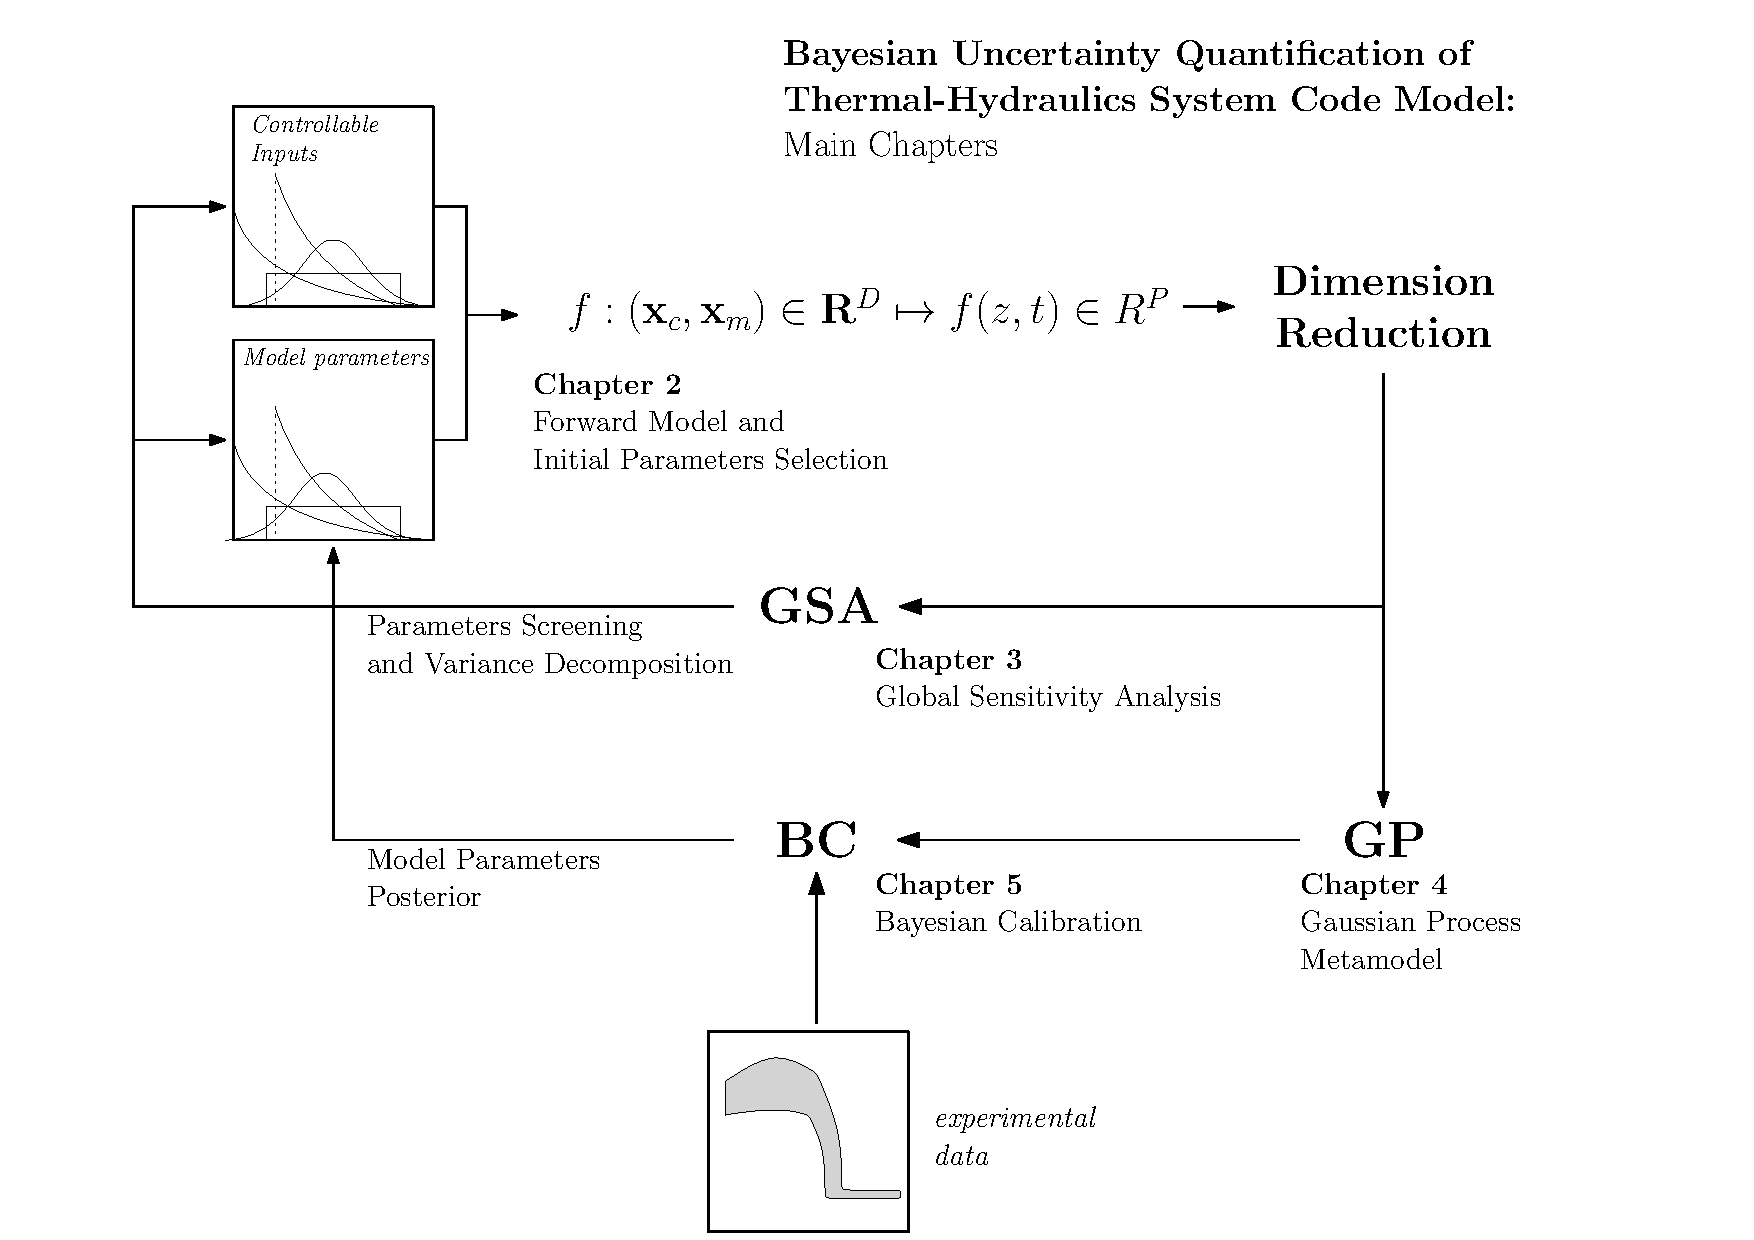
\includegraphics[width=\textwidth]{../figures/chapter1/figures/methodological_roadmap}
	\caption[The structure of thesis.]{The structure of the thesis, its main chapters.}
	\label{fig:ch1_methodological_roadmap}
\end{figure}

\textsc{Chapter~\ref{ch:trace_reflood}} gives an overview of the system thermal-hydraulics code \gls[hyper=false]{trace} with an emphasis on its reflood phenomena modeling and simulation.
The chapter also introduces the reflood experiment at the \gls[hyper=false]{feba} facility which serves as the experimental basis of this work followed by its modeling in \gls[hyper=false]{trace} code.
This model becomes the running case study in the three subsequent chapters to which the proposed methods are applied.
The chapter includes the selection of initial parameters relevant for reflood simulation and the propagation of their uncertainties on the code prediction.

\textsc{Chapter~\ref{ch:gsa}} introduces the \gls[hyper=false]{gsa} analysis methods adopted in this thesis with three key underlying ideas.
The first is to reduce the dimensionality of the code output space.
As the output of the simulation is time-dependent, dimension reduction is carried out while trying to preserve the interpretability of the results.
The second idea is to reduce the dimensionality of the input parameters space through parameter screening.
The third and final idea is to investigate, quantitatively, the effect of variation of parameters on the overall time-dependent output variation through variance decomposition.
The presented methods are then applied to the \gls[hyper=false]{trace} model of \gls[hyper=false]{feba} and the results are discussed. 

\textsc{Chapter~\ref{ch:gp_metamodel}} presents an approach to construct a fast surrogate model that approximates the inputs/outputs relationship of a computationally expensive simulator.
A minimum theoretical foundation of the method is first introduced, before moving on to describing an approach adapting the method for dealing with highly multivariate output via dimension reduction.
Afterward, the application of the method to the \gls[hyper=false]{trace} model of \gls[hyper=false]{feba} is presented and discussed.
In the end, a metamodel of the \gls[hyper=false]{trace} model is constructed and validated in anticipation of the high cost of the calibration approach presented in the following chapter.

\textsc{Chapter~\ref{ch:bayesian_calibration}}

\textsc{Chapter~\ref{ch:conclusions}}

%\begin{sidewaysfigure}
%	\centering
%	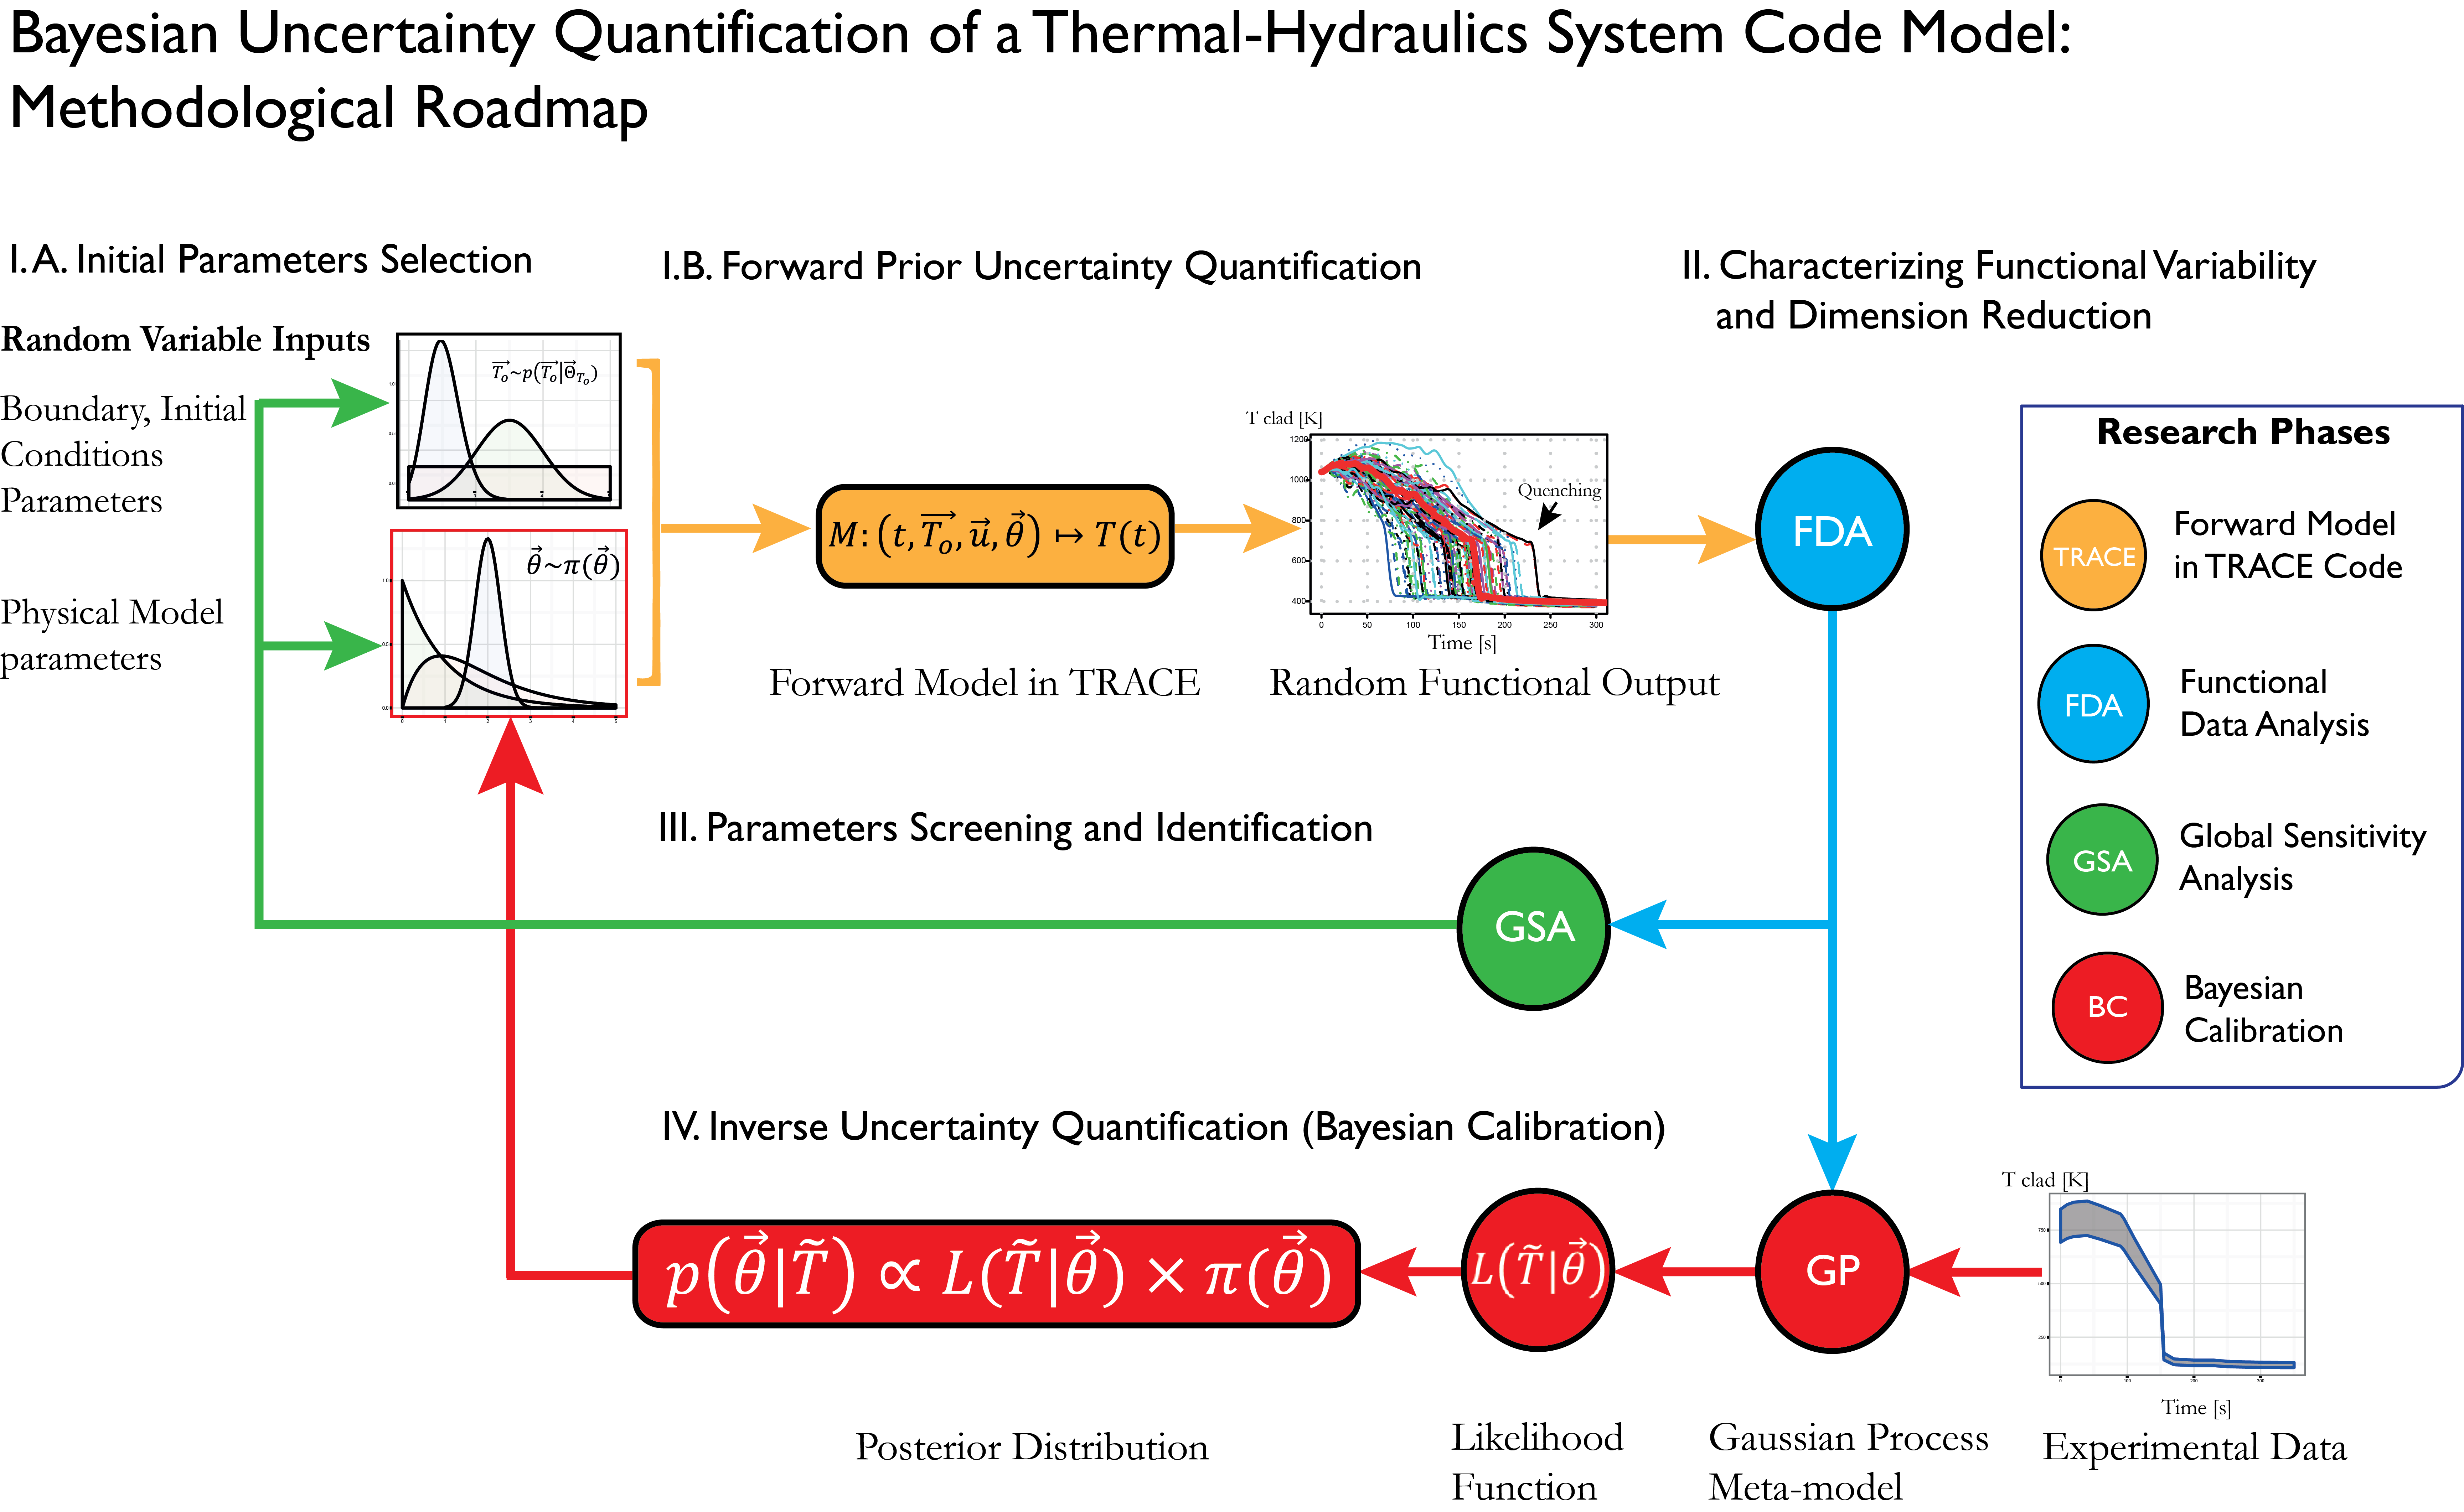
\includegraphics[width=0.85\textwidth]{../figures/methodologicalRoadmap/methodologicalRoadmap.pdf}
%	\caption{Methodological Roadmap of the Thesis}
%	\label{fig:methodological_roadmap}
%\end{sidewaysfigure}